\label{section:Formative_Study}

\subsection{Interviews with Professional Programmers}
To be informed of the system design, we conducted a formative interview study with five professional programmers (PA1--5, all male).
Because it is already well known how important code comprehension is in general, our interview focused on how they attempted to develop understanding and what issues they encountered.
All participants regularly used GitHub in their work environments.
This part of the formative studies revealed the following two findings.
%Our interview study took approximately one hour.
%The participants were offered a compensation of approximately 15 USD in the local currency at the end of the interview.
%As we conducted our interviews in a local language, we translated quotes in English for the following report.

\subsubsection{Burden for Collecting Development Contexts}
% In collaborative development, understanding code written by others is crucial.
% However, effort for code comprehension can be substantial. 
% PA1 stated how tedious it can be when he was involved in code review.

% % \myquote{(コードレビューにおいて、人のコードを読む事は)まじめにやるとコード書くのと同じくらい時間かかるんですよ}{P1}
% \myquote{(In code review,) Understanding others' code can be as time-consuming as writing code if you do it seriously.}{PA1}

Code comprehension includes understanding the context of how the code has been developed in addition to what it executes.
PA1 mentioned a particular issue related to code review caused by the lack of context understanding.

% \myquote{プロダクトの背景がわからないことが課題となっていて、長く見ている人が初めてそのチーム内でレビューできるようになっていて、まだやっぱり新入りの人がコードレビューできるような状況までドキュメントが整備されていないし、やっぱり背景理解が難しい。}{P1}
\myquote{One issue is the lack of background knowledge about the product. It makes only old members able to perform code review. Documentation is not ready for new members yet so that they can perform code review. It is still difficult for them to understanding the background.}{PA1}

% This problem becomes more prominent when new team members were on board.
% P1 mentioned that he frequently observed that new team members struggled on collecting background information.

% % \myquote{やっぱりコードの背景というか、コンテキストがわからないので、そこはなんかわかんないのは当たり前だと思う}{P1}
% \myquote{It is unsurprising that new team members do not understand the project well because they do not know its context or background.}{P1}

Such development contexts can also be useful for existing team members as PA3 stated:

% \myquote{どういう背景があってこのコードを実装したのかが書いてあると嬉しい。}{P3}
\myquote{It would be great if it is clear why this code has been implemented.}{PA3}

% Software documentation is one of the best practices to share knowledge of source code among team developers.
% However, PA5 stated that creating documentation would cause additional overhead in a project, and his team decided not to engage in it.

% % \myquote{チーム内でもドキュメントを作ろうという流れになる事はあります、ありますけど、正直なところあのーそこにさけるパワーは今、ちょっと・・、開発スピードを重視したいので}{P5}
% \myquote{We do have plans to create documentation, but to be honest, we don't have bandwidth for it now. We want to focus on speeding up our development.}{PA5}

\subsubsection{Pull Requests as an Information Resource}
% Code review was a common activity we observed in our interviews.
% It is one development process where a developer validates code revisions developed by another programmer.
% Bacchelli and Bird~\cite{MotivationOfCodeReview-Bacchelli} reported that while the main motivation for code review was to identify defects, reviewers also expected additional benefits, such as learning alternative solutions or performing knowledge transfer.
% For these multi-faceted benefits, code review becomes an integral part of a modern development process.

% GitHub supports code review through pull requests.
% A pull request includes a description of revisions as well as the actual code changes.
% A reviewer performs merge (or pull in GitHub) when she finds the revisions to be bug-free and legitimate.
% Our participants mentioned that additional effort by developers can greatly facilitate a code review process.
% For instance, a well-written description of a pull request can offer a sufficient amount of information about and reasons for the code changes, supporting reviewers' activities.

Our interview participants regularly used pull requests in their project as part of a code review process.
They agreed that comments and logs in pull requests can be useful to obtain information about code. 
For instance, PA3 and PA5 commented that he often referred to past pull requests to understand implementation reasons.

% \myquote{それは、実装を見ててこれってどういう意図でこうなってんのとかが、気になった時は、結構プルリクエスト上で議論がなされていることが多いので、それを探しに行くことはあります。}{P3}
\myquote{When I have a question about why this implementation was made, I look for pull requests because they often include related discussions.}{PA3}

%\myquote{僕はわりと探っちゃうタイプなので、昔どういうことあったんだろうみたいなのはまあ追っちゃう感じですね。}{P5}

\myquote{I like digging into code, so I often look for pull requests to see what happened in the past.}{PA5}

% PA1 and PA3 stated that they and their team explicitly described contexts as well as the content of changes.


% % \myquote{重要だと思ってるのは、まあ一個一個何でどういう目的でやるのかっていうのを書くようにしてるんですよね、formatをwhyとwhatを書くようにしている}{P1}
% \myquote{What's important to me is to describe what each change does for what purposes. We have a format (for pull requests) to make sure to write why and what.}{PA1}
% % \myquote{見てもらう人のことは考えて、どういう変更をどういう意図で行ったのかっていうのは、書くようにしている}{P3}
% \myquote{I always think of the reader, and clearly write what changes I have made for what purposes.}{PA3}

% Similar to general code comprehension, understanding development contexts is important for code review.
% P4 mentioned that the problem arises when he asked external developers to perform code review. 

% %\myquote{他のチームにレビューを頼む時に、プロダクトの背景がわからないことが課題となっていて、長く見ている人が初めてそのチーム内でレビューできるようになっていて、まだやっぱり新入りの人がコードレビューできるような状況までドキュメントが整備されていないし、やっぱり背景理解が難しい。}{P4}

% \myquote{When I have to ask someone in another team to review, the problem is that he does not have background knowledge about the project. People cannot do proper reviews until they are in a team for a long time.}{P4}

\subsection{Lab Study on Existing Command-based Approaches}

%Our interview with professional programmers revealed that past pull requests can be a useful resource for understanding code.
We conducted another formative study in our laboratory to understand how existing tools can support extraction of past pull requests.
%%%%%%%%%
% WWWWWWWWHYYYYYYYYYYYYYYYYYYY
% Specifically, we looked into tig\footnote{\url{https://github.com/jonas/tig}} and recursive-blame\footnote{\url{https://github.com/scottgonzalez/recursive-blame}}.
%%%%%%%%%%%%
To understand how these tools would be useful even for novice developers, we recruited seven university students (PB1 -- PB7) who had sufficient experience in GitHub and pull-request-based development.
We asked the participants to find pull requests related to portions of code in Chart.js given by the experimenter using tig and recursive-blame.
We then conducted a short interview to understand the user experience of these tools.


\subsubsection{Limited commit backtracking capability}

% P1 stated that recursive-blame often cannot trace back the history when the specified pattern of code was changed.

% % \myquoute{単純に名前が変わったりすると追えないとかがあるから、基本的にある程度あいまい検索ができるといいんだと思う}{P1}

% Tig finds the latest commit and version containing a change on the user-selected line of code using the git-blame command.
% However, it may fail to determine the commit when changes are substantial as P6 stated:

% \myquote{色々書きかえると結構すぐ追えなくなりますよね}{P6}

%The tools tested only take constrained input for search (a line of code and a regular expression or keyword in tig and recursive-blame, respectively).
%This limitation prevented our participants from correctly identifying relevant pull requests.
Our participants pointed out that existing tools cannot clearly inform whether the portion of interest was completely deleted or moved to a different part (e.g., by refactoring).
This is because the tools only show the deletion of such a portion and manual confirmation is necessary.

% \myquoute{違う名前や使い方が変わったときに、じゃあ何になったんだろうというってのを探すためには、前の名前しか知らないときは自分で探さないといけない。削除なのか、変更なのかわからないのが今のツールではわからない。}{P4}
\myquote{For example, when I found revisions on names or usage, I have to eyeball to figure out whether deletion or changes had occurred, which  these tools cannot tell me.}{P4}


\subsubsection{Limited interaction}
Although the two tools can identify past pull requests, their interfaces do not offer an overview of descriptions and comments.
This diminishes the utility of the tools as code comprehension support.
One of our participants commented that an overview of relevant pull requests would be desirable.

% \myquoute{全部やった後にさ、descriptionなかったらさ、なんやねーんって感じやん。多分descriptionが一番大事だから、はずれだったらすぐ次のを見せてほしい}{P2}
\myquote{I think descriptions are the most important. So I want to have a way to quickly move on to the next if the current pull request isn't useful.}{PB2}

% \myquoute{一度にいくつか(プルリクエストを)見られればうれしいかなと思う、まとめて勝手に深追いしてほしい}{P4}
\myquote{If I can see multiple pull requests at one time, that would be great. A system should just track back automatically.}{PB4}

%P5 wanted a system that simultaneously provides code and description in pull requests.
% \myquoute{コードと説明文の二つを同時に表示してあげるインタフェースがあると、使いやすいインターフェースかなと思うしとっつきやすいかなと思う}{P5}

Tig and recursive-blame take a single line of code and a regular expression or keyword for search, respectively.
Our participants complained that this search method does not fit to their expected use cases, and  the tools should support selection of multiple lines or code pieces.

% \myquoute{コード読んでて、この行だけわかんないってなることはないから}{P1}
\myquote{It's unlikely that I do not understand only this particular line when I read code.}{PB1}

% \myquoute{このifの中みたいな、意味のある単位で見たい。ifの行自体は別にそれほど興味ないし中身が大事かなみたいな}{P5}
\myquote{I want to look into a meaningful chunk, such as code inside this if block. I am not really interested in the line of the if statement itself.}{PB5}

%\subsubsection{Limited search capability}
% \myquoute{キーワードで検索は面倒というか、自分が思ったところを検索出来ているのか不安。どこが引っかかるか直感的じゃないから、tigのほうがいいかも}{P3}




\subsection{Summary}
Our interview studies highlight the following findings.

\begin{enumerate}
\setlength{\parskip}{1mm}
\setlength{\itemsep}{0mm}
%\item Developers are frequently required to understand codes before performing further actions (e.g., reviewing and making revisions).
\item Developers desire to obtain relevant information about the portion of code they are investigating for understanding, but they do not always have appropriate support.
\item Past pull requests can be useful to understand the context or reasons of code changes.
\item Existing tools, such as tig and recursive-blame, have limited capabilities on backtracking and interaction. In particular, existing methods would not work well for changes that involve relocation.
\end{enumerate}

These findings lead us to a hypothesis that supporting examination with past pull requests would be helpful to support comprehension of code portions though existing approaches are not easy to use.


% 		\begin{figure*}
%         \centering
%             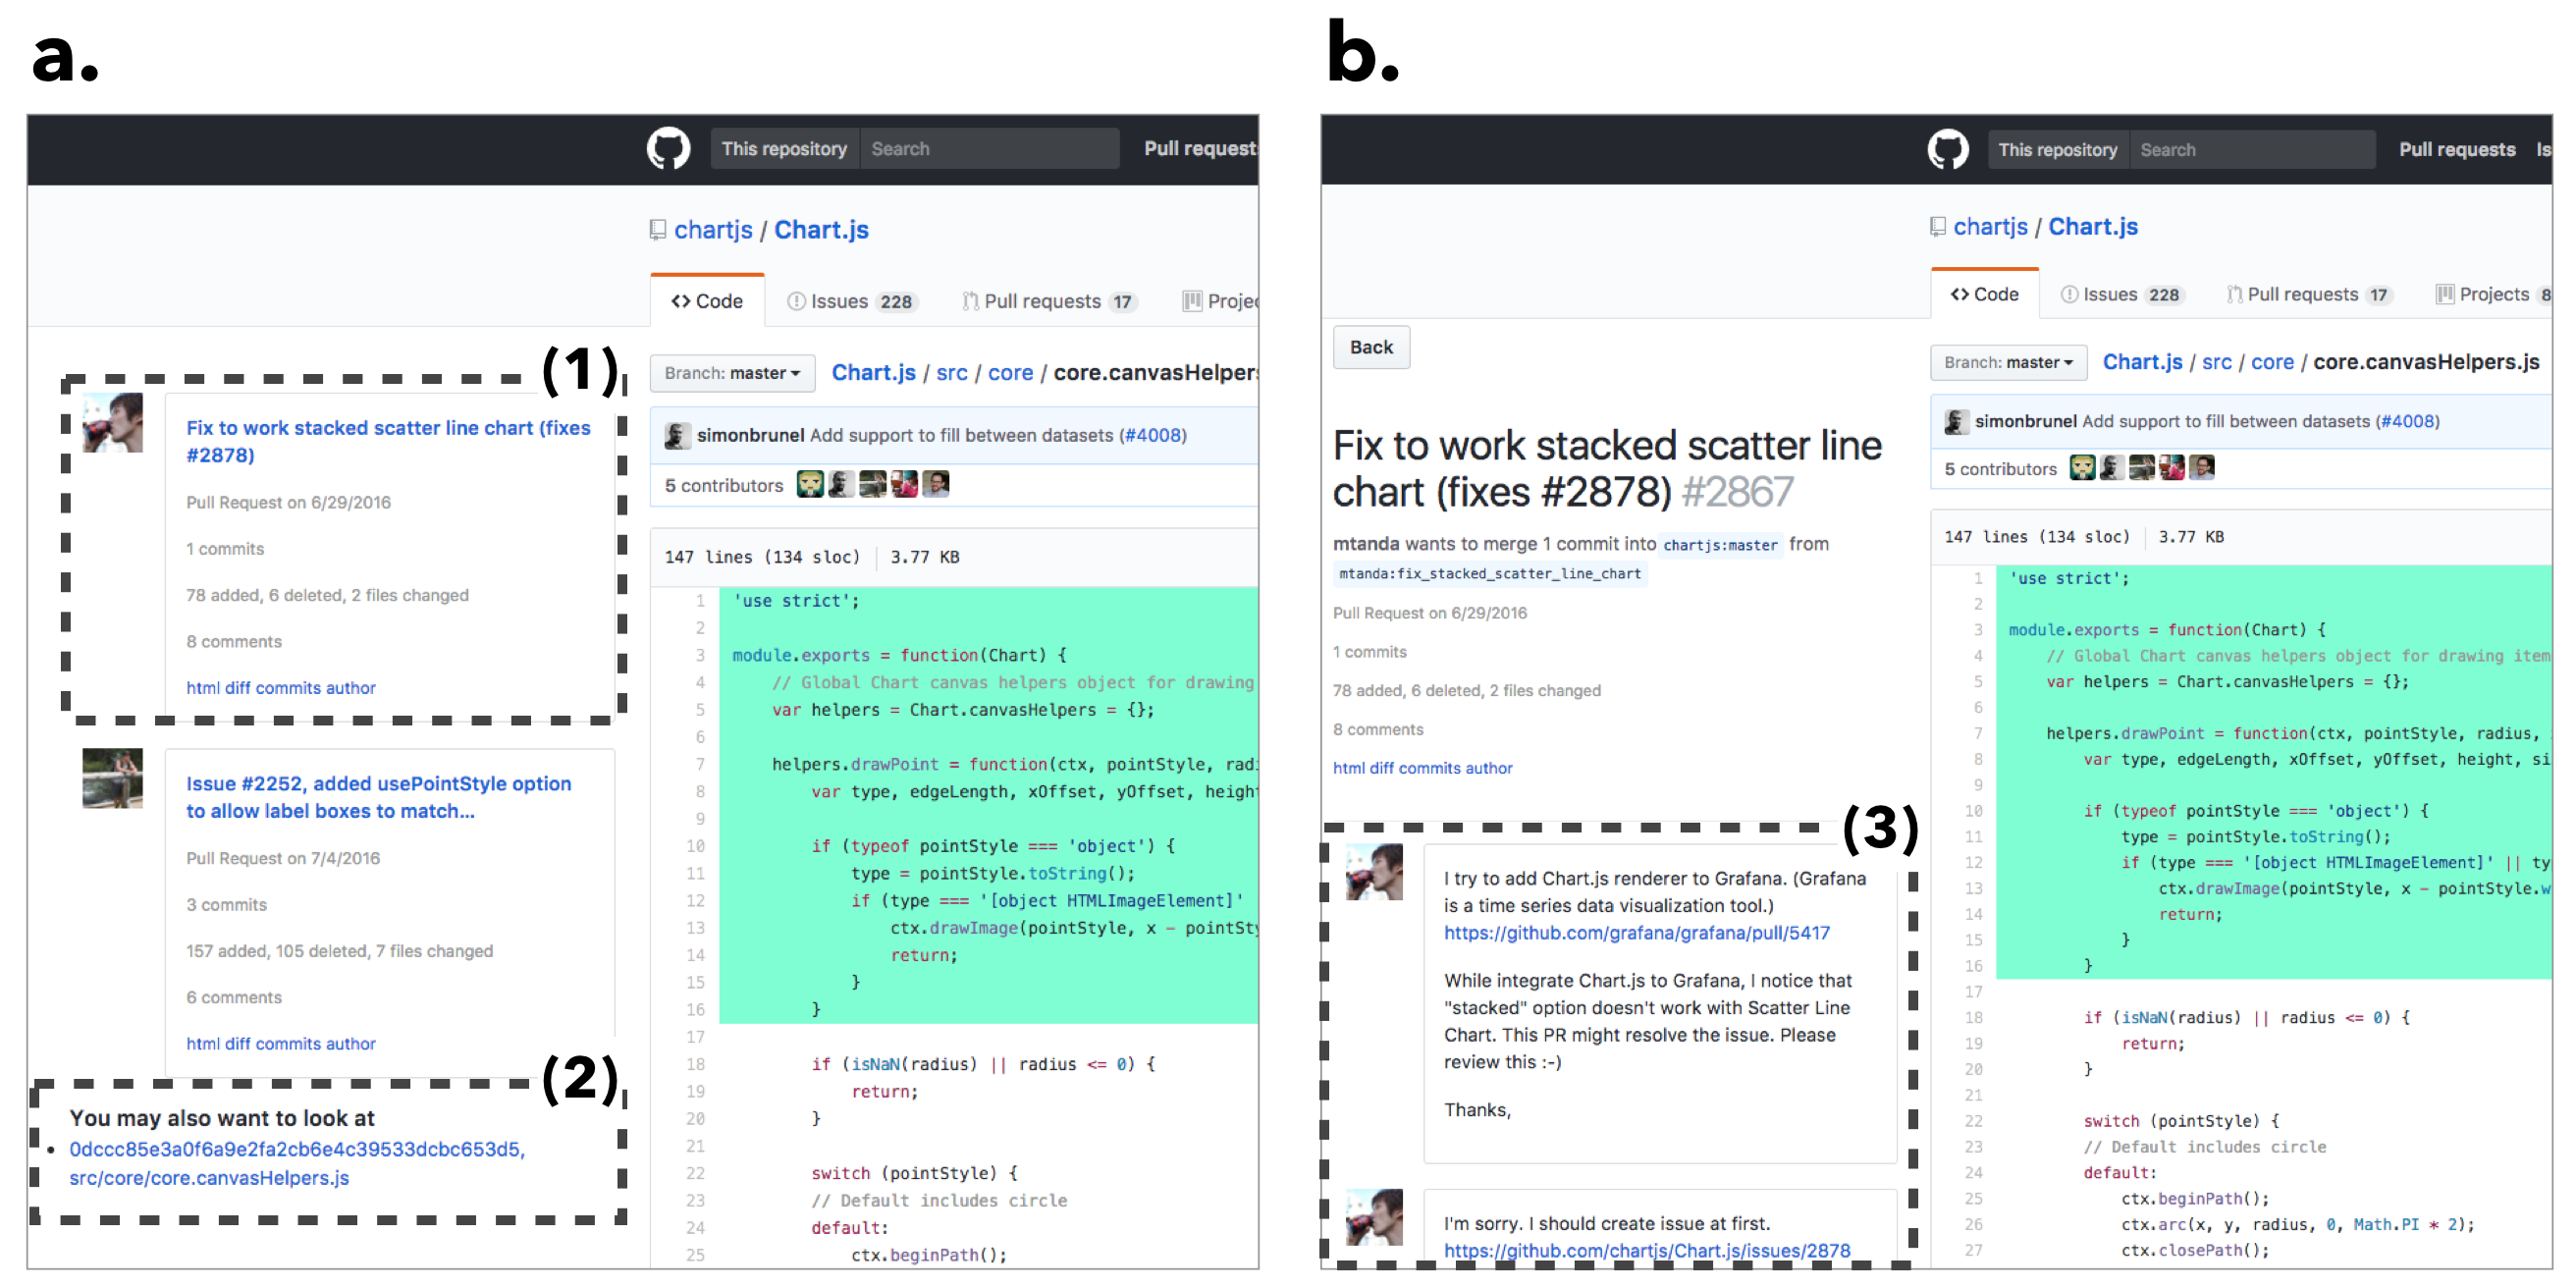
\includegraphics[width=2.0\columnwidth]{interface/CodeGlass.png}
%             \caption{The CodeGlass interface displays a series of pull requests associated with the selected code piece (highlighted in light green) in the chronological order. (1) Each pull request is summarized in a separate box. A summary shows the title of a pull request, its ID, and the numbers of commits, lines and files changed, and comments as well as links for additional information. (2) CodeGlass also suggests commits that are not included above but can be relevant if there exists any. When clicking one of them, the user can view the version associated with the selected commit and further investigate how code has been developed. (3) When the user clicks the title, CodeGlass presents review comments in the selected pull request.}~\label{fig:WebInterface}
%             \vspace{-5mm}
%       \end{figure*}
      
      
      
      

     